% Chapter 7 
% Last edit: 2017-5-4
\chapter[Statistical Intervals]{Statistical Intervals Based on a Single Sample}
\section{Basic Properties of Confidence Intervals}
$X_1,\dots,X_n \overset{iid}{\sim} f(x;\theta)$, use an interval to ``estimate" $\theta$.

\begin{exmp}
$X_1,\dots,X_n \overset{iid}{\sim} N(\mu,\sigma_0^2)$, $\sigma_0^2$ known.
\[\bar{X}\sim N\left(\mu,\frac{\sigma_0^2}{n}\right)\]
\[Z=\frac{\bar{X}-\mu}{\sigma_0/\sqrt{n}}\sim N(0,1)\]
\[P\left(-1.96\leq \frac{\bar{X}-\mu}{\sigma_0/\sqrt{n}} \leq 1.96 \right) =0.95\]
\[P\left(\bar{X}-1.96 \frac{\sigma_0}{\sqrt{n}} \leq \mu \leq \bar{X}+1.96 \frac{\sigma_0}{\sqrt{n}} \right) =0.95\]
So the chance that $\mu$ is within $\bar{x}\pm \frac{\sigma_0}{\sqrt{n}} $ is 95\%. Then we call $\left(\bar{X}-1.96 \frac{\sigma_0}{\sqrt{n}},\bar{X}+1.96 \frac{\sigma_0}{\sqrt{n}} \right)$ is the 95\% CI for $\mu$.
\end{exmp}

\subsection{Interpreting a Confidence Level}
Get 10000 such random samples independently, then 10000 different $\bar{X}$'s. Almost 9500 of such intervals will cover $\mu$.

\subsection{Other Levels of Confidence}

\begin{exmp}
A swimmer adopts a new swimming style. Historical data suggests that the time he needed to swim 200 metres is $\mu$ minutes within $0.5$ minutes s.d. He swims 9 times and the average he spent is 2.5 minutes. Suppose the swimming time is normally distributed. What is the 95\% CI for $\mu$?

\[X_1,\dots,X_9 \overset{iid}{\sim} N(\mu,0.5^2)\]
\[\bar{X}\pm 1.96 \frac{\sigma_0}{\sqrt{n}}=25 \pm 1.645 \frac{0.5}{\sqrt{9}}=2.5 \pm 0.274=(2.226,2.774) \]
the 97.5th percentile of $Z$ is 1.96 
\[P(Z \leq 1.96)=0.975\]
Denote $z_{0.025}=1.96$, as the 2.5th upper percentile of $Z$.
\end{exmp}

\begin{exmp}
The response time to do a command is normally distributed with $\sigma_0$= 25 ms. Want to estimate the $\mu$ for the system. How many times are necessary to assure that the 95\% CI for $\mu$ has a width at most 10 ms? 

95\% CI for $\mu$ is $\bar{X}\pm z_{\alpha/2} \frac{\sigma_0}{\sqrt{n}} $. Its width is $2 z_{0.025} \frac{25}{\sqrt{n}} \leq 10$.
\[\sqrt{n}\geq 9.8 \Rightarrow n\geq 96.04, \quad n=97\]

\end{exmp}

\begin{prop}
In general,
 \[P\left(-z_{\alpha/2} \leq \frac{\bar{X}-\mu}{\sigma_0^2/\sqrt{n}}  \leq  z_{\alpha/2} \right) = 1-\alpha\]
So $\bar{x} \pm  z_{\alpha/2} \frac{\sigma_0}{\sqrt{n}} $ is the $100(1-\alpha)\%$ CI for $\mu$.
\end{prop}

% Section 7.2
\section{Intervals Based on a Normal Population Distribution}
\noindent\fbox{%
    \parbox{\textwidth}{%
    \textbf{Assumption}
	
	The population of interest is normal, so that $X_1,\dots,X_n$ constitutes a random sample from a normal distribution with both $\mu$ and $\sigma$ unknown.
	}
}

\begin{theo}
$X_1,\dots,X_n \overset{iid}{\sim} N(\mu,\sigma^2)$, $\sigma$ unknown.
\[\frac{\bar{X}-\mu}{S/\sqrt{n}} \sim t(n-1)\]
where $S=\sqrt{\frac{1}{n-1} \sum_{i=1}^n (X_i-\bar{X})^2}$ is the sample s.d.

\begin{figure}[H]
\caption{t and Z distribution}
\centering
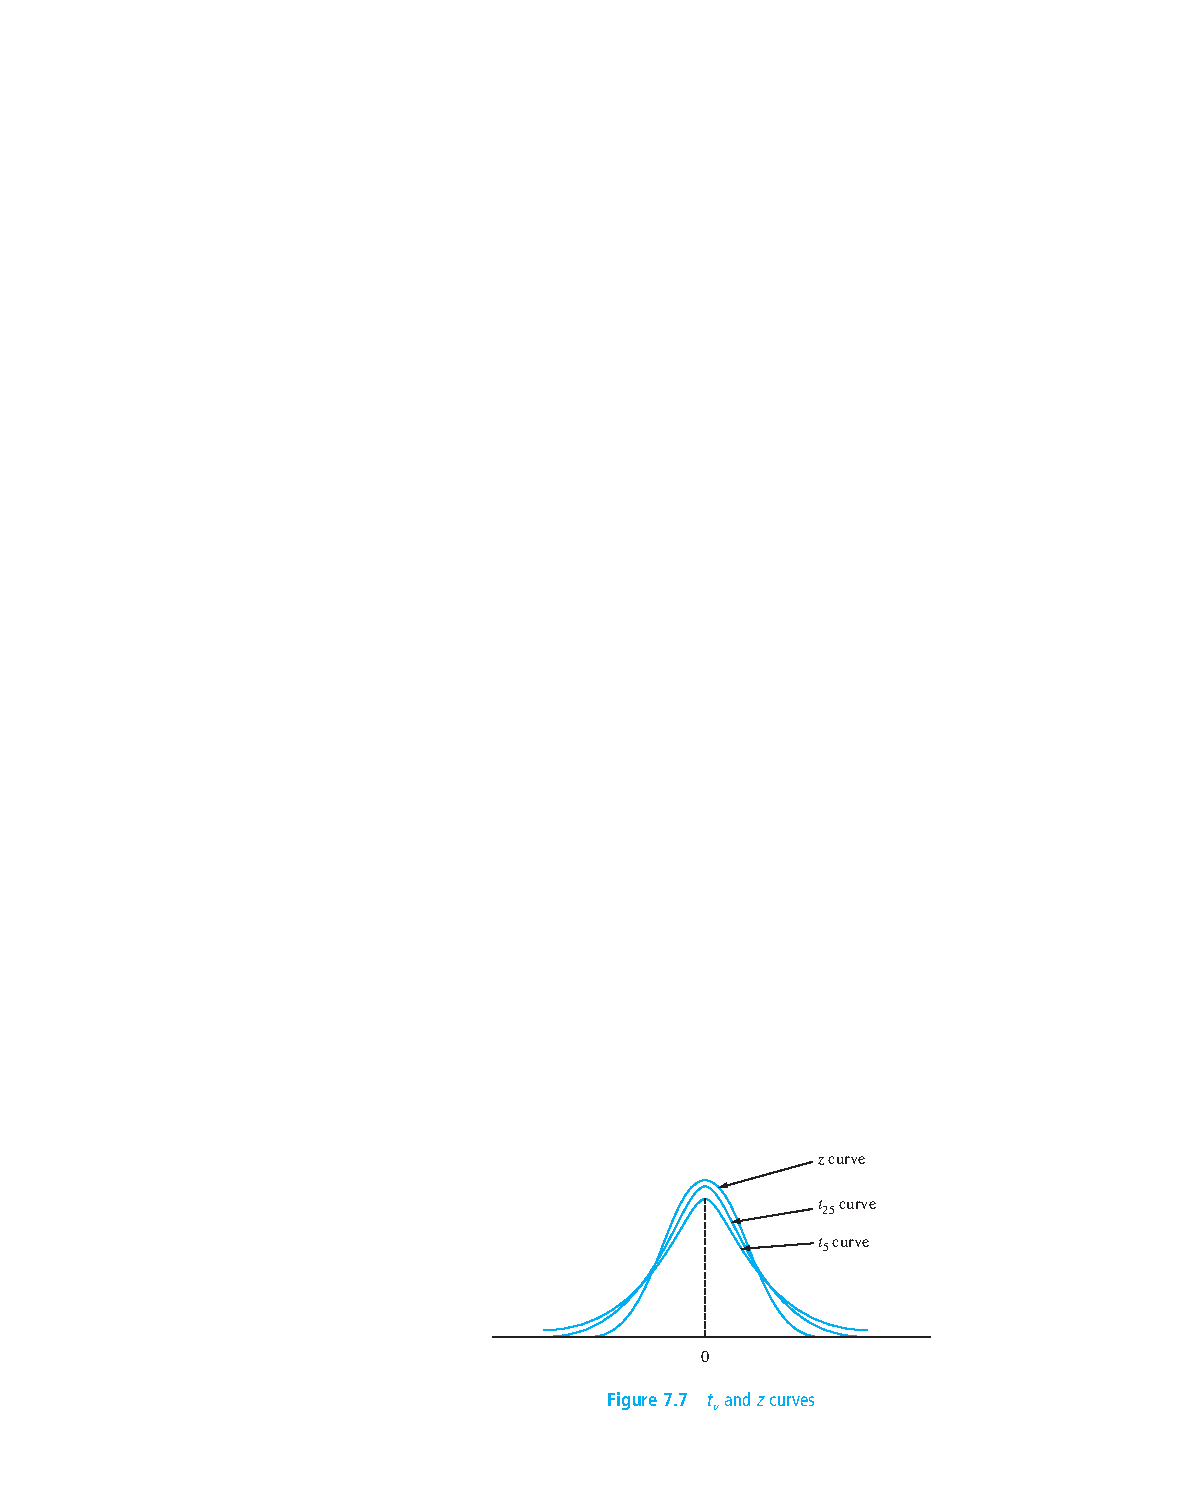
\includegraphics[scale=0.7]{t_distribution.png}
\end{figure}

\[P\left(-t_{\alpha/2,n-1} \leq \frac{\bar{X}-\mu}{S/\sqrt{n}}  \leq  t_{\alpha/2,n-1} \right) = 1-\alpha\]
where $t_{\alpha/2,n-1}$ denotes the $\frac{\alpha}{2}$-th upper percentile of $t(n-1)$.

Then $\bar{x} \pm  t_{\alpha/2,n-1} \frac{S}{\sqrt{n}} $ is the $100(1-\alpha)\%$ CI for $\mu$.
\end{theo}

\begin{exmp}
The following data are believed to be sampled from normal distribution. 10490, 16620, \dots, 14760 $(n=16)$

Then the 95\% CI for $\mu$ is 

\begin{align*}
\bar{x} \pm  t_{\alpha/2,n-1} \frac{S}{\sqrt{n}}=&14532.5 \pm  t_{0.025,15} \frac{2055.67}{\sqrt{16}}\\
=&(13437.3, 15627.7)
\end{align*} 

\end{exmp}
\subsection{A Prediction Interval for a Single Future Value}
See the corresponding text in the textbook.
\subsection{Tolerance Intervals}
See the corresponding text in the textbook.

% Section 7.3
\section{Large-Sample Confidence Intervals for a Population Mean and Proportion}
\subsection{A Large-Sample Interval for $\mu$}
\begin{prop}
$X_1,\dots,X_n \overset{iid}{\sim} (\mu,\sigma^2)$. $\mu$ and $\sigma$ are both unknown. By CLT if $n$ is large
\[\frac{\bar{X}-\mu}{S/\sqrt{n}} \overset{\cdot}{\sim} N(0,1)\]
\[P\left(-z_{\alpha/2} \leq \frac{\bar{X}-\mu}{S/\sqrt{n}}  \leq  z_{\alpha/2} \right) \overset{\cdot}{=} 1-\alpha\]

Then $100(1-\alpha)\%$ CI for $\mu$ is $\bar{x} \pm  z_{\alpha/2} \frac{s}{\sqrt{n}}$.
\end{prop}

\begin{exmp}
A random sample with $n=48$ is as follows 62, 50, 53,\dots, 50, 56, 58 with $n=48$, $\bar{x}=54.7$, $s=5.23$.

Then the 95\% CI for $\mu$ is 
\[54.7 \pm  z_{0.025} \frac{5.23}{\sqrt{48}}=(53.2, 56.2)\]
\end{exmp}

\subsection{How to Construct a Confidence Interval In General}
$X_1,\dots,X_n \overset{iid}{\sim} f(x;\theta)$. Want to construct a confidence interval for $\theta$
\begin{enumerate}
\item Find a statistic (pivot) which depends on $X_1,\dots,X_n $ and $\theta$ only;
\item Its distribution does not depend on $\theta$ or any other unknown parameters.
\end{enumerate}

\subsection{A General Large-Sample Confidence Interval}
$X_1,\dots,X_n \overset{iid}{\sim} f(x;\theta)$ and $\hat{\theta}$ is an estimate.
For $\theta$, satisfying 
\begin{enumerate}
\item approximately normal 
\item is approxiamtely unbiasd
\item $\sigma_{\hat{\theta}}^2=Var(\hat{\theta})$ is available
\end{enumerate}

Then
\[P\left(-z_{\alpha/2} \leq \frac{\hat{\theta}-\theta}{\sigma_{\hat{\theta}}}  \leq  z_{\alpha/2} \right) = 1-\alpha\]

\subsection{A Confidence Interval for a Population Proportion}
\begin{exmp}
A random sample of $n$ individual is selected from $Bern(p)$. $p=$ success rate.
\[X_1,\dots,X_n \overset{iid}{\sim} Bern(p)\]
\[\boxed{Var(X_i)=p(1-p)  \qquad \hat{p}=\bar{X}}\]
\[Y=\sum_{i=1}^n X_i \sim Bin(n,p)\]

$\hat{p}=\frac{Y}{n}$ is an estimate for $p$. By CLT,
\[\frac{\sqrt{n}(\hat{p}-p)}{\sqrt{p(1-p)}} \overset{\cdot}{\sim} N(0,1)\]
\[P\left(-z_{\alpha/2} \leq \frac{\sqrt{n}(\hat{p}-p)}{\sqrt{p(1-p)}}  \leq  z_{\alpha/2} \right) \overset{\cdot}{=} 1-\alpha\]

So, $100(1-\alpha)\%$ CI for $p$ is $\hat{p} \pm  z_{\frac{\alpha}{2}} \sqrt{\frac{p(1-p)}{n}}$, but $p$ is unknown.
\end{exmp}

\textbf{Remedy}
\begin{enumerate}
\item If $n$ is large, replace $p$ by $\hat{p}$ in the CI formula
$\hat{p} \pm  z_{\frac{\alpha}{2}} \sqrt{\frac{\hat{p}(1-\hat{p})}{n}}$
\item 
\[P\left(-z_{\alpha/2} \leq \frac{\sqrt{n}(\hat{p}-p)}{\sqrt{p(1-p)}}  \leq  z_{\alpha/2} \right) \overset{\cdot}{=} 1-\alpha\]
\[p-z_{\alpha/2}\sqrt{\frac{p(1-p)}{n}} \leq\hat{p}\leq p+z_{\alpha/2}\sqrt{\frac{p(1-p)}{n}} \]
\[(p-\hat{p})^2 \leq z_{\alpha/2}^2 \frac{p(1-p)}{n} \]

Solving the quadratic equation for $p$.
\[\frac{\hat{p}+\frac{z_{\alpha/2}}{2n} \pm z_{\alpha/2}\sqrt{\frac{\hat{p}(1-\hat{p})}{n}+\frac{z_{\alpha/2}^2}{4n^2}}}{1+z_{\alpha/2}^2 /n}\]

is the $100(1-\alpha)\%$ CI for $p$.
\end{enumerate}

\subsection{One-Sided Confidence Intervals (Confidence Bounds)}
\[X_1,\dots,X_n \overset{iid}{\sim} N(\mu,\sigma_0^2)\]
\[P\left(\frac{\bar{X}-\mu}{\sigma_0/\sqrt{n}} \leq z_{\alpha}\right)=1-\alpha\]
Then $P\left(\mu\leq \bar{X}+z_{\alpha}\frac{\sigma_0}{\sqrt{n}}\right)=1-\alpha$. So $\bar{X}+z_{\alpha}\frac{\sigma_0}{\sqrt{n}}$ is the $100(1-\alpha)\%$ upper confidence bound for $\mu$. Similarly, $\bar{X}-z_{\alpha}\frac{\sigma_0}{\sqrt{n}}$ is the $100(1-\alpha)\%$ lower confidence bound for $\mu$. $P\left(\mu\geq \bar{X}-z_{\alpha}\frac{\sigma_0}{\sqrt{n}}\right)=1-\alpha$.

If $\sigma$ is unknown, $\bar{X}+t_{\alpha,n-1}\frac{\sigma_0}{\sqrt{n}}$ is the $100(1-\alpha)\%$ upper confidence bound for $\mu$. $\bar{X}-t_{\alpha,n-1}\frac{\sigma_0}{\sqrt{n}}$ is the $100(1-\alpha)\%$ lower confidence bound for $\mu$.

If large sample, $\bar{x}+z_{\alpha}\frac{s}{\sqrt{n}}$, $\bar{x}-z_{\alpha}\frac{s}{\sqrt{n}}$.

\begin{exmp}
(Example 7.10 in the textbook)
\end{exmp}

\begin{exmp}
37 helmets are tested. 24 of them shown damage: let $p$ denote the proportions of all helmets showing damage under the same impact condition.
\begin{enumerate}
\item Caculate 99\% CI for $p$.
\item What sample size is required for the width of 99\% CI to be at most 0.1?
\end{enumerate}
\textbf{Solution.}

(1) $X=\text{\# of helmets with damages}\sim Bin(37,p)$.
Observe $x=24$, $\hat{p}=\frac{x}{n}=\frac{24}{37}$.

MM: $E(X)=np$, then $n\hat{p}=X$, $\hat{p}=\frac{X}{n}$

MLE: $L(p)= \binom {37}{x} p^x (1-p)^{37-x}$
\[l(p)=\log{\binom {37}{x}}+x \log{p}+(37-x)\log{(1-p)}\]
\[l'(p)=0 \qquad \hat{p}=\frac{x}{n}=\frac{24}{37}\]
\[\hat{p}=\frac{X}{n}\overset{\cdot}{\sim} N\left(p,\frac{p(1-p)}{n}\right)\]
99\% CI for $p$ is $\hat{p} \pm  z_{0.005} \sqrt{\frac{\hat{p}(1-\hat{p})}{n} }=(0.4465,0.8507)$.

(2) Width of 99\% CI is 
\[2 z_{0.005} \sqrt{\frac{\hat{p}(1-\hat{p})}{n} } \leq 0.1\]
\[n \geq \left(\frac{2\times 2.575}{0.1}\right)^2 \hat{p}(1-\hat{p})\]
\[n\geq \left(\frac{2\times 2.575}{0.1}\right)^2 \cdot\frac{1}{4}\]
\end{exmp}

% Section 7.4
\section{Confidence Intervals for the Variance and Standard Deviation of a Normal Population}
\begin{theo}
Then $X_1,\dots,X_n$ are a random sample from $N(\mu,\sigma^2)$. Then
\[\frac{(n-1)S^2}{\sigma^2} \sim \chi^2(n-1)\]
\end{theo}

Then
\[P\left(\chi^2_{1-\alpha/2,n-1} \leq \frac{(n-1)S^2}{\sigma^2} \leq \chi^2_{\alpha/2,n-1} \right)=1-\alpha\]

So $100(1-\alpha)\%$ CI for $\sigma^2$ is
\[\left(\frac{(n-1)s^2}{\chi^2_{\alpha/2,n-1}}, \frac{(n-1)s^2}{\chi^2_{1-\alpha/2,n-1}} \right)\]

Then $100(1-\alpha)\%$ CI for $\sigma$ is
\[\left(	\sqrt{\frac{(n-1)s^2}{\chi^2_{\alpha/2,n-1}}}, \sqrt{\frac{(n-1)s^2}{\chi^2_{1-\alpha/2,n-1}}}\right)\]


\begin{exmp}
(Example 7.15 in the textbook)
\end{exmp}